
\documentclass{article}
\usepackage[utf8]{inputenc}
\setlength{\parskip}{5pt} % esp. entre parrafos
\setlength{\parindent}{0pt} % esp. al inicio de un parrafo
\usepackage[spanish]{babel}
\usepackage[sort&compress,numbers]{natbib} % referencias
\usepackage[top=25mm,left=20mm,right=20mm,bottom=25mm]{geometry} % margenes
\usepackage{graphicx} % poner figuras
\usepackage{color,listings}
\usepackage{tikz}
\usepackage{minted}
\usepackage{caption}
\usepackage{subcaption}
\usetikzlibrary{automata,topaths}
\renewcommand\lstlistingname{Código}
\title{P6}
\author{Ismael Crespo}
\date{\today}

\begin{document}

\maketitle

\section{Introducción}
El contenido de este trabajo presenta la simulación numérica de una epidemia basado en elementos que pueden ser Infectados($I$), Susceptibles ($S$) y Recuperados($R$), las infecciones se dan al inicio de manera pseudoaleatoria entre la población y después al existir una convivencia (distancia euclidiana corta) los elementos sanos pueden infectarse, una vez infectados después de un determinado número de pasos es posible que un elemento sea recuperado y genere inmunidad. Se analiza el impacto en el desarrollo de la pandemia en relación al aislamiento (reducción de la movilidad de los infectados) y la inmunidad desarrollada por una vacunación en el inicio de la pandemia. La creación de este análisis se realizó creando rutinas en \emph{R 4.1.2}. Los efectos de la reducción en la movilidad y la vacunación se realizan modificando el código desarrollado por E. Schaeffer \citep{E.Schaeffer}
\section{Objetivos}
1.-Estudia el efecto de contención en el sentido de que agentes infectados reduzcan su velocidad de movimiento a la mitad durante su infección. Determina con pruebas estadísticas adecuadas si este cambio produce un efecto significativo en la magnitud de la epidemia (la altura del pico en la curva del porcentaje de infectados por iteración) y en la velocidad de ella (la iteración en la cual se llega por la primera vez al valor pico).

2.-Vacunar con probabilidad $pv$ a los agentes al momento de crearlos de tal forma que están desde el inicio en el estado $R$ y ya no podrán contagiarse ni propagar la infección. Estudia el efecto estadístico del valor de $pv$ (de cero a uno en pasos de 0.1) en el porcentaje máximo de infectados durante la simulación y el momento (iteración) en el cual se alcanza ese máximo.

\section{Programación en R}
La simulación de la pandemia se basa en asignar caracteres ($I$,$S$ y $R$) al número de elementos propuestos en la variable $n$. En función a la probabilidad $pi$ un elemento en estado inicial $S$ pasará a estar en estado $I$, un elemento en estado $S$ se va a contagiar con una probabilidad de contagio $pc$ que esta en función de la distancia euclidiana entre los elementos. Los elementos se mueven en una velocidad aleatoria para cada caso en una región delimitada a $x=1$ y $y=1$ y esta velocidad, $dx$ y $dy$ en cada paso, es una fracción de la longitud en $x$ y $y$ asignada aleatoriamente el código P6 en la referencia [1] realiza la rutina descrita. El código \ref{R1} muestra como se asignan los factores $I$, $R$ y $S$, para la primera parte del trabajo se muestra como la velocidad se reduce dividiendo entre la variable $movilidad$ la velocidad asignada al inicio a los elementos que son infectados al inicio y conforme avanza la epidemia. El día en el que se llega al pico se obtiene utilizando la funicón \texttt{which.max}.





\lstset{basicstyle=\ttfamily, keywordstyle=\bfseries}
\begin{lstlisting}[frame=single,numbers=left,language=R,caption=Asignación de los factores para los elementos y reducción de la velocidad con la variable $movilidad$ para los elementos infectados \label{R1}]
 movilidad=c(1,2,3,4)
for( mov in movilidad){
for(repeticion in 1:rep){
agentes <- data.frame(x = double(), y = double(),
                      dx = double(), dy = double(),
                      estado  = character())
for (i in 1:n) {
    e <- "S"
    if (runif(1) < pi) {
        e <- "I"
    }
for(i in 1:n){
        if(agentes$estado[i] == "I"){
         agentes$dx[i]=agentes$dx[i]/mov
         agentes$dy[i]=agentes$dy[i]/mov 
 }}

\end{lstlisting}  
Para el efecto de la vacunación los elementos son vacunados, al inicio de la epidemia en función de la probablidad $pv$, la vacuna asignara el factor $R$ a los elementos para generar una inmunidad ante los infectados. La movilidad no se modifico para evaluar solamente el efecto de la vacunación. Para ambos analisis de vacunación y movilidad se realizaron 10 replicas y fueron analizadas por medio de diagramas caja-bigote (véase el código \ref{R1.1}).
\lstset{basicstyle=\ttfamily, keywordstyle=\bfseries}
\begin{lstlisting}[frame=single,numbers=left,language=R,caption=Vacunación en función de $pv$ para generar inmunidad al inicio de la epidemia. \label{R1.1}]
for(pv in seq(0.0,1 , by = 0.1))
for (i in 1:n) {
    e <- "S"
     vacuna=runif(1)
     if (runif(1) < pi) {
        e <- "I"
     }
     if ( vacuna< pv) {
        e <- "R"
    }
\end{lstlisting}


\section{Resultados}
La figura \ref{F2}  presenta el impacto que tiene la reducción de la movilidad, similar a lo que ofrece el aislamiento, de los elementos infectados en la pandemia, en la figura \ref{fig2a} se analiza el porcentaje de infectados en el pico de la pandemia según el nivel de aislamiento al que fueron sometidos los elementos infectados, en la figura \ref{fig2b} se observa el día en el que se llegó al pico de la pandemia. La figura  \ref{fig2c} y la figura \ref{fig2d} presentan la curva de la pandemia en el caso de que la movilidad no se restringe para los casos infectados y para cuando la movilidad se restringe en $1/4$ de su movilidad original. Los resultados muestran una clara reducción en los contagios y una epidemia con forma de meseta alargada durante los 100 días de simulación para la reducción de la velocidad a $1/4$ de la original cuando se es infectado . En las secuencias gráficas del desarrollo de las epidemias de la figura \ref{F2}, disponibles en como material complementario en el repositorio de la practica \citep{REPOP6}, se observa como los elementos infectados al reducir su velocidad no llevan la infección, los contagios se dan solo por aquellos que se acercan a ellos.

\begin{figure}
     \begin{subfigure}[]{.4\linewidth}
         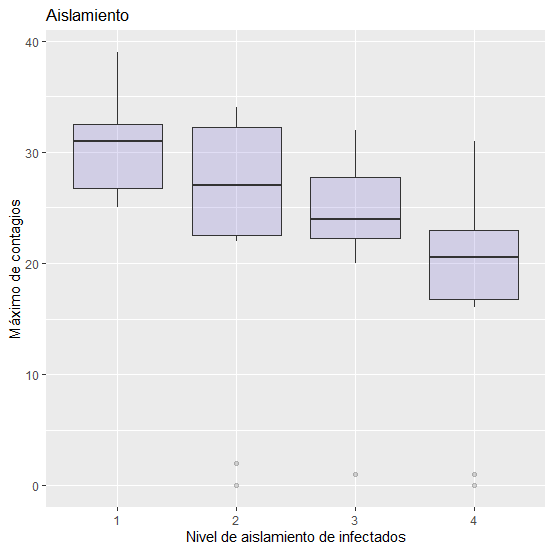
\includegraphics[width=\linewidth]{p6_infectados.png}
         \caption{Porcentaje de infectados según la restricción de la movilidad de los infectados.}
         \label{fig2a}
     \end{subfigure}
     \begin{subfigure}[]{.4\linewidth}
         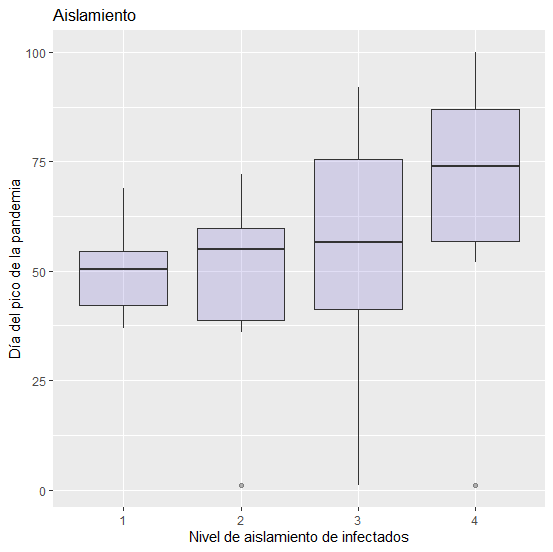
\includegraphics[width=\linewidth]{p6_dia.png}
         \caption{Día en el que se llega al pico de la pandemia según la restricción de la movilidad de los infectados.}
         \label{fig2b}
     \end{subfigure}
     \begin{subfigure}[]{.5\linewidth}
     \centering
         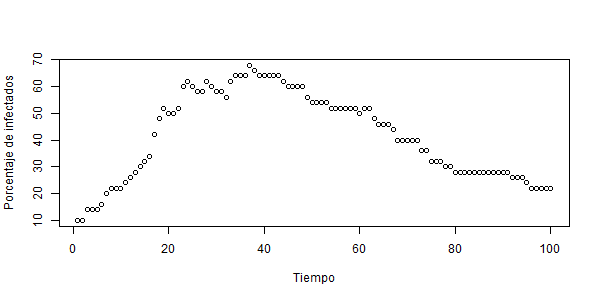
\includegraphics[width=\linewidth]{p6_1.png}
         \caption{Curva de la pandemia sin restricción de movilidad.}
         \label{fig2c}
     \end{subfigure}
     \begin{subfigure}[]{.5\linewidth}
     \centering
         \includegraphics[width=\linewidth]{p6e_4.png}
         \caption{Curva de la pandemia con restricción a $1/4$ de movilidad.}
         \label{fig2d}
     \end{subfigure}
     \caption{Desarrollo de las pandemia en función de la movilidad de los infectados.}
        \label{F2}
\end{figure}
En la figura \ref{F3} se presenta el mismo análisis del máximo de contagios y el día en el que se llega al pico de la pandemia variando $pv$ que determina el alcance de la vacunación en un estado inicial para desarrollar inmunidad a una fracción de la población ante posibles infecciones, el valor de $pv$ varia de 0 a 1, interpretamos a 0.1 como una vacunación muy deficientes y a 1 como una vacunación universal. En la figura \ref{3a} se presenta el máximo de contagios en relación a la vacunación y la figura \ref{3b} presenta el día en el que se llega al pico de la pandemia, la figura \ref{3c} y la figura \ref{3d} presentan el comportamiento de la pandemia para la vacunación cuando $pv=0.2$ y $pv=0.7$. En las secuencias gráficas del desarrollo de las epidemias de la figura \ref{F3}, disponibles en como material complementario en el repositorio de la practica \citep{REPOP6}, se observa el comportamiento de la población cuando hay inmunidad entre la población al inicio de la pandemia.
\begin{figure}
     \begin{subfigure}[]{.4\linewidth}
         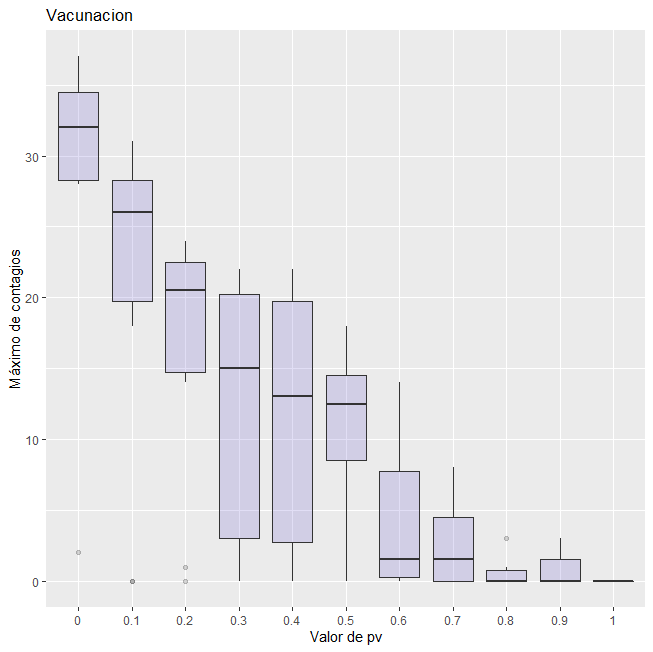
\includegraphics[width=\linewidth]{p6_infectados_r1.png}
         \caption{Máximo de contagios en función de la vacunación.}
         \label{3a}
     \end{subfigure}
     \begin{subfigure}[]{.4\linewidth}
         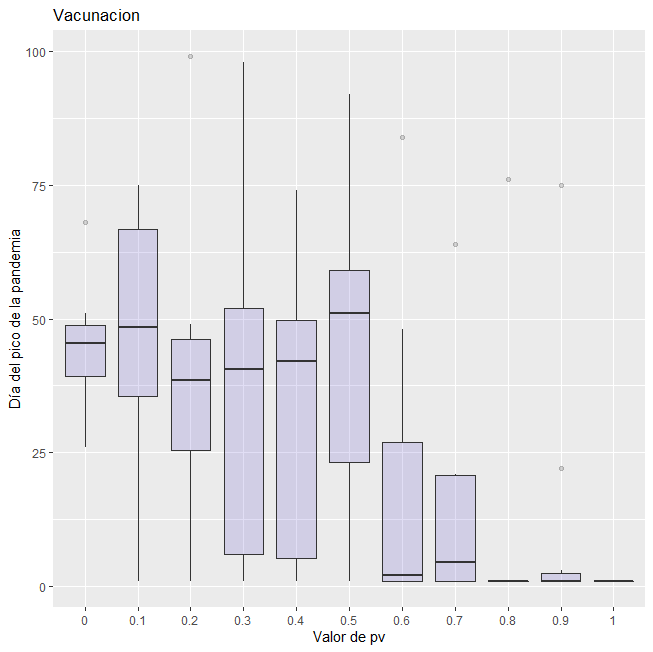
\includegraphics[width=\linewidth]{p6_dia_r1.png}
         \caption{Día del pico de la pandemia en función de la vacunación.}
         \label{3b}
     \end{subfigure}
     \begin{subfigure}[]{.5\linewidth}
     \centering
         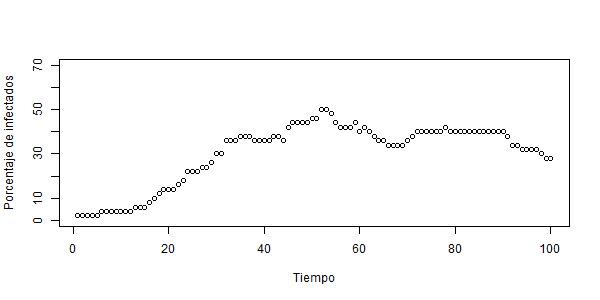
\includegraphics[width=\linewidth]{p6_r1_0.2.png}
         \caption{Curva de la epidemia $pv=0.2$.}
         \label{3c}
     \end{subfigure}
       \begin{subfigure}[]{.5\linewidth}
       \centering
         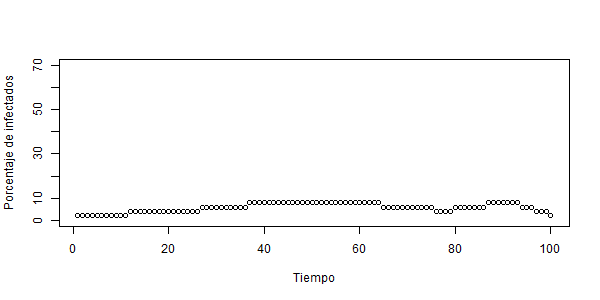
\includegraphics[width=\linewidth]{p6_r1_0.7.png}
         \caption{Curva de la pandemia $pv=0.7$.}
         \label{3d}
     \end{subfigure}
     \caption{Desarrollo de la pandemia en función del nivel de vacunación.}
        \label{F3}
\end{figure}

\section{Conclusiones}
Tanto la reducción en la movilidad como la vacunación son métodos efectivos para controlar la pandemia, se destaca la vacunación como el método mas efectivo cuando se consigue un alcance importante de la vacunación dentro de la población, sin embargo el aislamiento ofrece una herramienta para contener el contagio sin necesidad de una campaña de vacunación cuando no se tiene acceso a esta.
\bibliography{simu}
\bibliographystyle{plainnat}
\end{document}
